\documentclass[10pt, brown]{beamer}
\usetheme{Warsaw}
\usepackage[MeX]{polski}
\usepackage[cp1250]{inputenc}  % Polskie literki...
\usepackage[polish]{babel}     %
\usepackage{parskip}
\usepackage{latexsym,gensymb,amsmath,amssymb,amsthm}
\usepackage{graphicx}
%\usepackage{verbatim}
\usepackage{ragged2e}
\usepackage{url}
%\setlength{\parindent}{0pt}
%\setlength{\parskip}{1ex}
\renewcommand{\qedsymbol}{$\square$}
\newenvironment{dowod}{{\bf Dow�d.}}{\hfill\rule[0.025cm]{0.21cm}{0.21cm}}
\newtheorem{tw}{Twierdzenie}
\newtheorem{fakt}{Fakt}
\newtheorem{lemat}{Lemat}
\newtheorem{wn}{Wniosek}

\author{dr in�. Jakub Mo�aryn, mgr in�. Jan Klimaszewski}
\institute{Instytut Automatyki i Robotyki}
\date{Warszawa, 2018}
\title{Sterowanie mechanizm�w wielocz�onowych}
\subtitle{Wyk�ad 2 - standardowe modele uk�ad�w wielocz�onowych}
\begin{document}
%
\frame{
\titlepage
}
%
\section{Manipulator RRR}
%
\frame{
    \frametitle{Model kinematyki}
}
%
\frame{
    \frametitle{Zadanie proste kinematyki}
}
%
\frame{
    \frametitle{Zadanie odwrotne kinematyki}
}
%
\frame{
    \frametitle{Zadanie proste kinematyki pr�dko�ci}
}
%
\frame{
    \frametitle{Zadanie odwrotne kinematyki pr�dko�ci}
}
%
\frame{
    \frametitle{Model dynamiki}
}
%
\section{Acrobot}
%
\frame{
    \frametitle{Model kinematyki}
    \begin{columns}[T] % align columns
        \begin{column}{.48\textwidth}
            \begin{figure}[htb!]
                \begin{center}
                    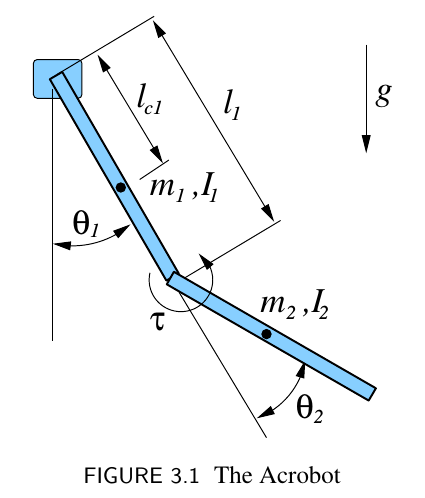
\includegraphics[width=0.9\linewidth]{../../figures/acrobot}
                    %\\[1em]%
                    \caption{acrobot} \label{fig:acrobot}
                \end{center}                                         
            \end{figure}
        \end{column}%
        
        \hfill%
        
        \begin{column}{.48\textwidth}
            Przyjmujemy:\\
            $\theta_1, \theta_2$ - wsp�rz�dne maszynowe.\\
            $q = [\theta_1,\theta_2]^T, x=[q,\dot{q}]^T$
        \end{column}%
    \end{columns}
}
%
\frame{
    \frametitle{Zadanie proste kinematyki}
    
    \begin{equation}
        x_1 =
        \begin{bmatrix}
            l_1 s_1 \\
            -l_1 c_1 \\
        \end{bmatrix}
        , x_2 = x_1 + 
        \begin{bmatrix}
            l_2 s_{12} \\
            -l_2 c_{12} \\
        \end{bmatrix}
        .
    \end{equation}
}
%
\frame{
    \frametitle{Zadanie odwrotne kinematyki}
}
%
\frame{
    \frametitle{Zadanie proste kinematyki pr�dko�ci}
}
%
\frame{
    \frametitle{Zadanie odwrotne kinematyki pr�dko�ci}
}
%
\frame{
    \frametitle{Model dynamiki (1)}
    The energy2 is given by: 
    \begin{align}
        T = T_1 + T_2 \\
        T_1 = \frac{1}{2}I_1\dot{q_1}^2 \\
        T_2 = \frac{1}{2}(m_2 l_1^2 + I_2 + 2 m_2 l_1 l_{c2} c_2)\dot{q_1}^2 + \frac{1}{2}I_2\dot{q_2}^2 + (I_2 + m_2 l_1 l_{c2} c_2)\dot{q_1}\dot{q_2}\\
        U = -m_1 g l_{c1} c_1 - m_2 g (l_1 c_1 + l_2 c_{12})
    \end{align}
    
    Entering these quantities into the Lagrangian yields the equations of motion:
    \begin{align}
        \nonumber
        (I_1 + I_2 + m_2 l_1^2 + 2 m_2 l_1 l_{c2} c_2) \ddot{q_1} + (I_2 + m_2 l_1 l_{c2} c_2) \ddot{q_2} - 2 m_2 l_1 l_{c2} s_2 \dot{q_1} \dot{q_2} \\
        - m_2 l_1 l_{c2} s_2 \dot{q_2}^2 + (m_1 l_{c1} + m_2 l_1) g s_1 + m_2 g l_2 s_{12} = 0 \\
        (I_2 + m_2 l_1 l_{c2} c_2)\ddot{q_1} + I_2 \ddot{q_2} + m_2 l_1 l_{c2} s_2 \dot{q_1}^2 + m_2 g l_2 s_{12} = \tau
    \end{align}
}
%
\frame{
    \frametitle{Model dynamiki(2)}
    
    In standard, manipulator equation form, we have:

    \begin{align}
        H(q) = 
        \begin{bmatrix}
            I_1 + I_2 + m_2 l_1^2 + 2 m_2 l_1 l_{c2} c_2    &   I_2 + m_2 l_1 l_{c2} c_2 \\
            I_2 + m_2 l_1 l_{c2} c_2                        &   I_2 \\
        \end{bmatrix} \\
        C(q, \dot{q}) = 
        \begin{bmatrix}
            - 2 m_2 l_1 l_{c2} s_2 \dot{q_2}                &   - m_2 l_1 l_{c2} s_2 \dot{q_2} \\
            m_2 l_1 l_{c2} s_2 \dot{q_1}                    &   0 \\
        \end{bmatrix} \\
        G(q) = 
        \begin{bmatrix}
            (m_1 l_{c1} + m_2 l_1) g s_1 + m_2 g l_2 s_{12} \\
            m_2 g l_2 s_{12} \\
        \end{bmatrix} \\
        B = 
        \begin{bmatrix}
            0 \\
            1 \\
        \end{bmatrix}
    \end{align}
}
%
\section{Wahad�o odwr�cone}
%
\frame{
    \frametitle{Model kinematyki}
}
%
\frame{
    \frametitle{Zadanie proste kinematyki}
}
%
\frame{
    \frametitle{Zadanie odwrotne kinematyki}
}
%
\frame{
    \frametitle{Zadanie proste kinematyki pr�dko�ci}
}
%
\frame{
    \frametitle{Zadanie odwrotne kinematyki pr�dko�ci}
}
%
\frame{
    \frametitle{Model dynamiki}
}
%

\end{document}
